\documentclass[conference]{IEEEtran}
\usepackage{graphicx}
\usepackage{amsmath}
\usepackage{amssymb}
\usepackage{amsxtra}
\usepackage{amstext}
\usepackage{latexsym}
%\usepackage{dsfont}
\usepackage{float}
\usepackage{cite}
\usepackage{subcaption}
\usepackage{epstopdf}
\usepackage{caption}
\ifCLASSINFOpdf
  % \usepackage[pdftex]{graphicx}
  % declare the path(s) where your graphic files are
  % \graphicspath{{../pdf/}{../jpeg/}}
  % and their extensions so you won't have to specify these with
  % every instance of \includegraphics
  % \DeclareGraphicsExtensions{.pdf,.jpeg,.png}
\else

\fi
\hyphenation{op-tical net-works semi-conduc-tor}
\begin{document}
\title{Influence of Polarization Direction on Static \\ On-Body Propagation Channels}
\author{Lingfeng~Liu$^1$, Peng~Zhang$^1$, Xiaonan~Wang$^1$, Chaoqun~Wang$^2$\\
\\
$^1$School of Information Engineering, East China Jiaotong University, China \\
$^2$School of Information Engineering,  Nanchang University, China}
%\address{$^1$School of Information Engineering, East China Jiaotong University, China \\
%$^2$School of Information Engineering, East China Jiaotong University, China\\

%\small Email: Author@XXX.XXX
%}
\maketitle
\begin{abstract}
On-body propagation channels show significant polarization selectivity in static and dynamic scenarios. In this work, we measured polarized on-body channels on static body at 2.4 GHz by monopole antennas, where standing and sitting postures are considered. The polarization direction of the antenna (Z-polarization, H-polarization, V-polarization) depends on the the direction of the antenna in the body position. In the statistical characteristics of the channels, the V-polarization direction of the receiving antenna is more conducive to receiving signal and reducing the path losses. Cross-polar discrimination (XPD) are calculated from measurement data, the strongly depolarization of on-body channels is more easily caused by the human sitting posture due to legs scattering. No matter how the polarization direction of the transmission antenna , the receiving antenna can generally obtain a decent field component in the V-polarization direction.
\end{abstract}
%\begin{keywords}

%\end{keywords}
%\IEEEpeerreviewmaketitle
\section{Introduction}
On-body communications in wireless body area networks (WBANs) are short distance communications defined on or above the body of limited height \cite{1}. An essential feature of on-body propagation channels is that they do not follow conventional far-field propagation principles and exhibits complex near-field characteristics including the body scattering effects\cite{2,3} and surface wave propagation \cite{5}. Studies as \cite{6} have shown the high sensitivity of on-body channels to the orientation of the transmit and receiving antennas, implying a possible polarization diversity for ultra-low powered sensor communication in e.g. medical and wearable applications. 

Earlier studies on the finite-difference-time-domain (FDTD) simulations of the electromagnetic fields on the body surface \cite{} have shown that due to the near-field body scattering effects, the surface wave propagation assumption may not fully consistent with the actual wave propagation in on-body channels, resulting the channel polarization dispersion both along and normal to the propagation path defined. The postures and body dynamics will further lead to the variation of the on-body polarization distribution over time and space domains. One limitation of previous measurements as reported in \cite{6,7} is that most of the measurements cover partial polarization configurations of on-body channels. Consequently, the polarization matrix of the channels are not fully characterized and modeled. Full-space description of the channel polarization distribtuion under specific scenarios is necessary to correctly capture the field components of the on-body channels. 

In this work, measurements of polarized narrowband on-body channels at 2.4 GHz on static human body are conducted in indoor environment. Full polarization configuration are investigated for channels covering the key parts of the body. Two static postures of the body, i.e. the standing and sitting postures, were invesitgated, and the cchannel polarization distribution under the two postures were compared. The polarization matrix and the cross polarization descrimination (XPD) matrix for each scenario are summarized. The polarization gain and the depolarization ratio of the investigated on-body channels are invstigated.

This paper is organised as follows. Section \ref{sec:setup} describe the configuration of the measurements. Section \ref{sec:analysis} present the statistical analysis of the channel polarization distribution and depolarization characteristics. Finally, section \ref{sec:conslusion} summarize the analysis. 


\section{Measurement Settings}\label{sec:setup}

\begin{figure}[!t]
  \centering
  \begin{subfigure}[t]{0.3\textwidth}
  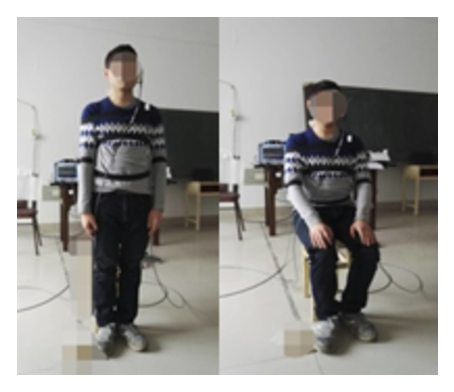
\includegraphics[width=\textwidth]{figs/1a.eps}
  \label{fig:volunteer}
  \end{subfigure}
  \begin{subfigure}[t]{0.25\textwidth}
  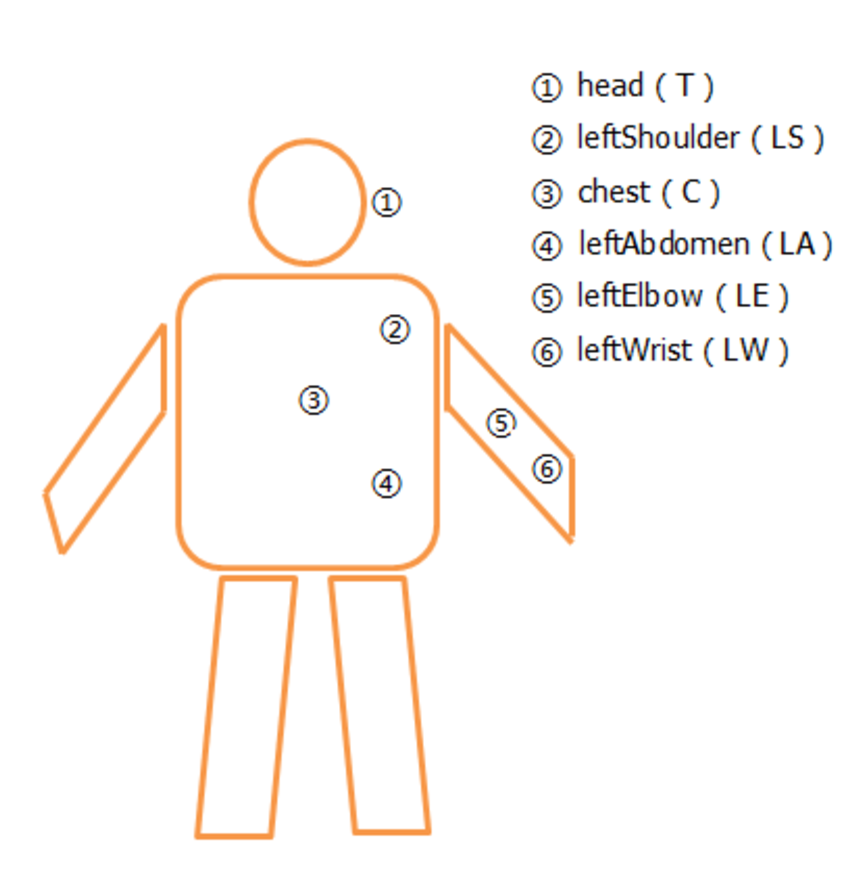
\includegraphics[width=4.5cm,height=5cm]{figs/1b.eps}
  \label{fig:placement}
  \end{subfigure}
  \begin{subfigure}[t]{0.19\textwidth}
  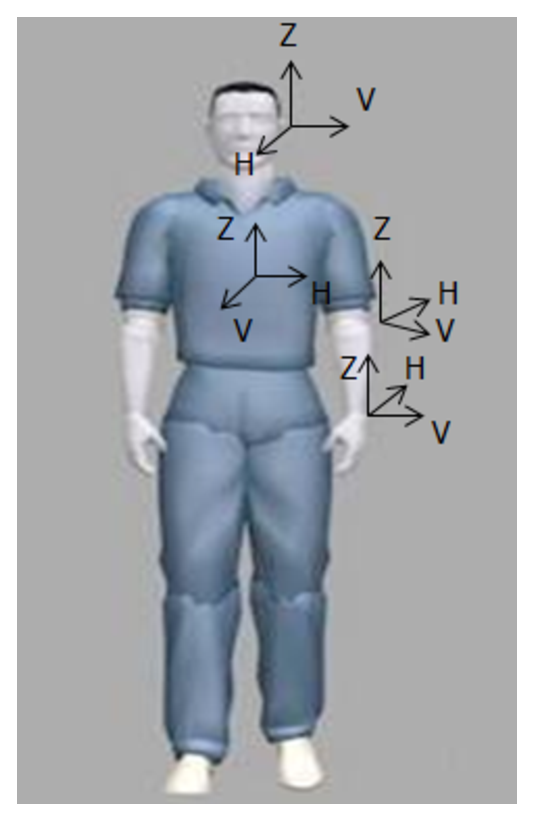
\includegraphics[width=3cm,height=5cm]{figs/1c.eps}
  \label{fig:polarization_direction}
  \end{subfigure}
\caption{Measurement context at 2.4 GHz. (a) Indoor scenario and human body postures. (b) Node placement on the body. (c) The definition of Polarization direction in different parts of the body.}
\label{fig:human}
\end{figure}

The measurements were carried out in an indoor environment of an empty laboratory in dimension of 6 by 7 meters, no large obstacles around. 

A male volunteer of height 160 cm and weight 50 kg was chosen. Two postures, standing and sitting with arms naturally posed, are investigated as shown in Fig. \ref{fig:volunteer}. On-body channels were selected based on 5 key parts of the body as presentd in Fig. \ref{fig:placement}, which are head-left-shoulder (T-LS), head-left-wrist (T-LW), chest-left-abdomen (C-LA), left-shoulder-chest (LS-C), and left-elbow-left-wrist (LE-LW) channels. We assume the environment as reflection neglegible, and the channels is primarily affected by their geometry distribution and body scattering.

We investigated narrowband on-body channels at 2.4 GHz frequency band over time domain. To avoid heavy interference from the Wi-Fi signals, the actual A vector network analyzer (VNA) of type R\&S ZVB 20 was applied to measurement the channel S-parameters over time domain. 
VNA is set to 2.484 GHz continous wave frequency, the antenna is a vertical polarization monopole antenna. The specific settings of VNA and antenna are shown in Table \ref{tab:1}. The antennas were mounted 2cm above the body surface to avoid body coupling effect. The actual measured frequency is 2.484 GHz to avoid the intense usage of WiFi channels. We investigated five group of on-body channels, , respectively. The key parts of the body such as the Fig.\ref{fig:1}(b), different combinations of which allow establishing useful communication links, such as a head-mounted display or a wrist-mounted input device. The impact of ground reflection is minimized due to these links in the upper half of the body.\par
\begin{table}[!t]
\centering
\captionsetup{labelsep=newline}
\caption{RADIO SETTINGS}
\label{tab:1}
%\subcaption{VNA setting}
\begin{tabular}{cc}
\hline
Parameter&Value\\
\hline
VNA&ROHDE SCHWAR ZNB 20\\
The number of points&1000\\
Power&10 dBm\\
IF bandwidth&10 KHz\\
Sweeptime&auto(10s)\\
\hline
Antenna&Monopole\\
Frequency bands&2.4 GHz\\
Range&2.4-2.5 GHz\\
Impedance&50 ohm\\
Regulations&ISM\\
\hline
\end{tabular}
\end{table}
\begin{table}[!t]
\centering
\captionsetup{labelsep=newline}
\caption{PATH LOSS(dB)}
\label{tab:2}
\scalebox{0.75}{
\begin{tabular}{cccccccccc}
\hline
Standing Set&ZZ&ZV&ZH&VZ&VV&VH&HZ&HV&HH\\
\hline
T-LS&37.18&25.39&27.81&29.74&23.60&28.83&41.04&28.98&26.72\\
T-LW&58.11&37.21&47.69&59.12&42.78&61.49&61.84&48.39&62.10\\
C-LA&65.36&36.70&48.95&49.86&29.90&39.78&63.44&36.34&54.88\\
LS-C&50.38&30.32&43.70&49.68&30.69&54.65&54.81&35.68&45.71\\
LE-LW&47.66&23.92&31.12&42.14&29.99&29.93&50.10&30.33&27.97\\
\hline
Stitting Set&ZZ&ZV&ZH&VZ&VV&VH&HZ&HV&HH\\
\hline
T-LS&35.58&26.75&27.67&23.84&23.65&34.50&29.66&27.75&24.80\\
T-LW&53.47&39.17&39.60&58.62&47.17&46.49&58.22&39.24&43.51\\
C-LA&43.84&40.94&50.46&46.75&25.34&38.79&38.53&33.60&41.84\\
LS-C&47.02&30.60&48.15&50.81&31.09&50.89&45.27&36.66&46.30\\
LE-LW&39.05&35.77&32.07&44.11&28.52&32.32&56.16&33.52&25.91\\
\hline
\end{tabular}}
\end{table}
For near-field propagation, the direction of field may not follow the vertical relationship with the propagation direction due to the interaction between the radiation source and the body scattering. This will cause field spreading in all directions. To facilitate the study of on-body channels, the antenna��s orientation is defined relative to the body surface in 3 directions, vertical tangential to the body, denoted as Z, horizontal tangential to the body, denoted as H, vertical normal to the body, denoted as V. The polarizations are defined differently in different parts of the body because of the irregularity of the shape of the body, as shown in Fig.\ref{fig:1}(c). Consequently, for one scenario investigated, the channel is measured in total of 9 polarization combinations, denoted as XY, \begin{math}X.Y\in\{Z,V,H\},\end{math} where X is the polarization of the transmit antenna and Y is the receiving antenna polarization. The measurements are found to maintain flat fading during the measurement, hence the mean of the channel is investigated.


\section{Measurement Statistical Analysis}\label{sec:analysis}

\subsection{Receiving V-polarization}
The average path loss of on-body channels in different polarization combinations are presented in the Table \ref{tab:2}. In the standing posture, the optimal polarization combination of T-LS and C-LA channels is VV, and the optimal polarization combination of T-LW, LS-C and LE-LW channels is ZV. In the sitting posture, the optimal polarization combination of the other channels does not change, except for the LE-LW channel (HH). This shows that the V-polarization direction of the receiving antenna may capture the major part of the signal waves. On the contrary, V-polarization is not found at the receiving side by analyzing the worst polarization combinations of on-body channels. Such as the worst combination of T-LS and C-LB channels is ZZ in the standing posture. Although the worst polarization combinations of the T-LW and LS-C channels contain the V-polarization direction in the sitting posture, it is not at the receiving side. These indicate that the V-polarization of the receiving antenna plays a significant role in reducing the path losses and effectively receiving signal.\par
\begin{figure}[!t]
  \centering
  % Requires \usepackage{graphicx}
  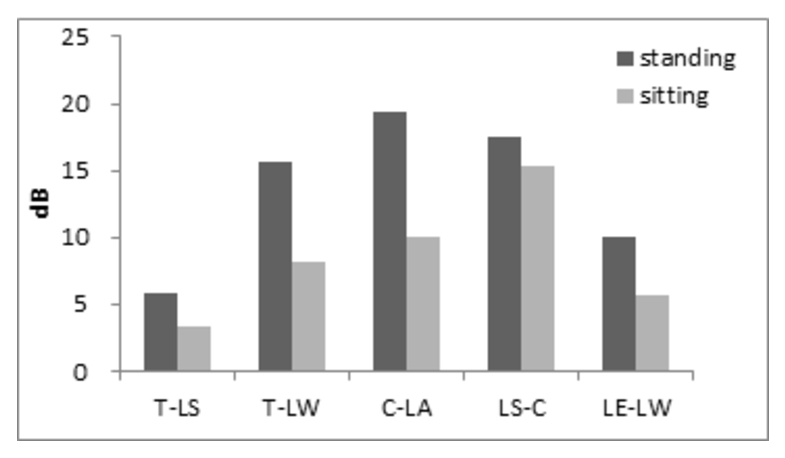
\includegraphics[width=0.4\textwidth]{figs/2.eps}\\
  \caption{The gain of receiving V-polarization of each channel in different postures.}
  \label{fig:2}
\end{figure}
\begin{figure*}[!t]
\centering
\begin{subfigure}[t]{\textwidth}
%\centerline{
\centering
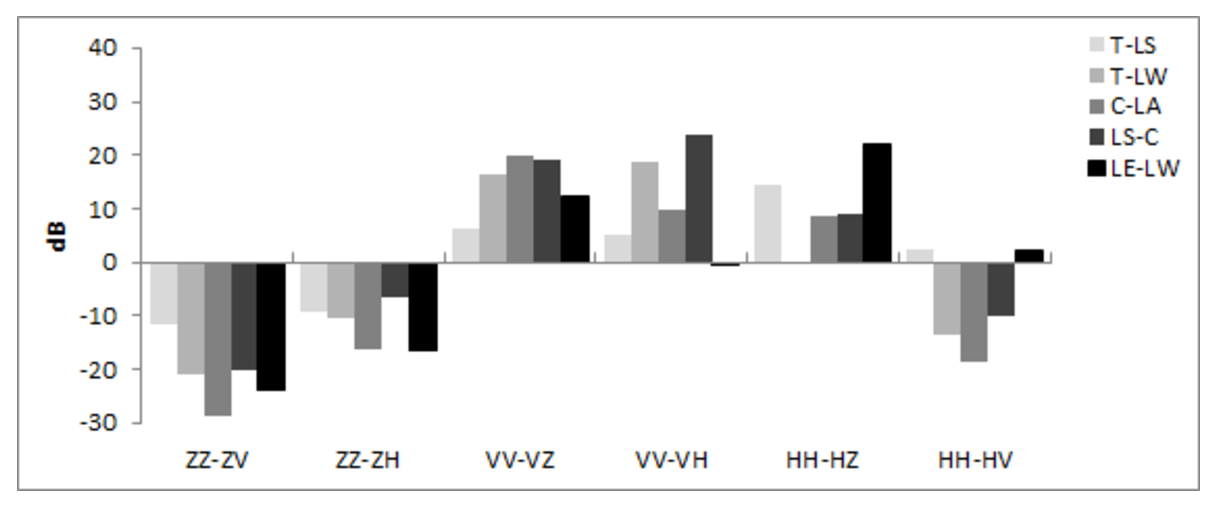
\includegraphics[width=14cm,height=4cm]{figs/3a.eps}
\subcaption{}
\label{fig:3a}
\end{subfigure}
\begin{subfigure}[t]{\textwidth}
\centering
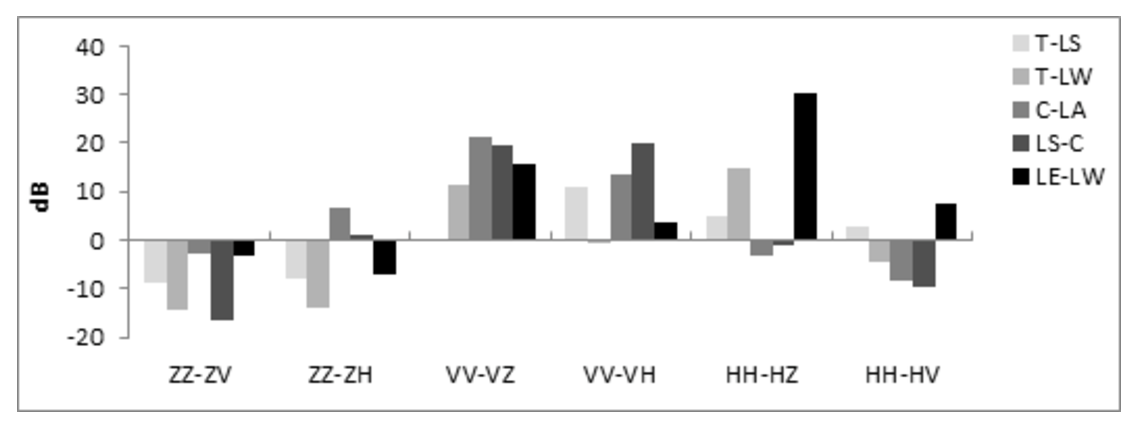
\includegraphics[width=14cm,height=4cm]{figs/3b.eps}
\subcaption{}
\label{fig:3b}
\end{subfigure}
\caption{XPD of on-body channels in six scenarios. (a) XPD in the standing posture. (b) XPD in the sitting posture.}
\label{fig:3}
\end{figure*}
Since the V-polarization direction making the antenna perpendicular to the body surface extending outward, which reduces the scattering of the body surface to the radiation source and the absorption of energy by the body. The Z and H polarization directions of the antenna maintain a parallel relationship with the human body, making the impact of body scattering on the radiation source is stronger than V direction. As a result, field propagating along the body surface will orient its field along the perpendicular direction than the other directions. The receiver in V-polarization can receive the  major part of the signal waves caused by the interaction between the body scattering and the field source.
\subsection{polarization gain}
To more specifically describe the advantages of the V-polarization of the receiving antenna, we define the gain of receiving V-polarization as
\begin{equation}\label{ep:1}
G_{R_{V}}=\frac{\sum\limits_I\sum\limits_J{\textbf{PL}(IJ)}}{6} -\frac{\sum\limits_I{\textbf{PL}(IV)}}{3}
\end{equation}
where \begin{math}I\in\{Z,H,V\}, J\in\{Z,H\}\end{math}, IJ and IV represent polarization combination, \textbf{PL}(IJ) is the path loss of IJ polarization combination, \textbf{PL}(IV) is the path loss of IV polarization combination.
The  V-polarization gain of each channel is shown in Fig.\ref{fig:2}. The V-polarization gain of the standing posture is better than that of sitting in each channel. The V-polarization gain of each on-body channel is at least 5dB in the standing posture. In addition, the gain of each channel can also reach at least 3dB in the sitting posture.
\subsection{Channel depolarization}
As the polarizations described in Section II were defined with respect to the body surface orientation at the antenna position. The body scattering effect leads to heavy cross polarization that will cause the field polarization become away from the polarization as defined. The de-polarization is studied by the following six scenarios. The change of the Z polarization into V and H directional components at the receive antenna can be characterized by comparing ZZ and ZV combinations (scenario ZZ-ZV), ZZ and ZH combinations (scenario ZZ-ZH). De-polarization from the V-polarization into Z and H polarization is characterized by VV and VZ combinations (scenario VV-VZ), VV and VH combinations (scenario VV-VH). Similarly, comparing the HH and HZ combinations (scenario HH-HZ), HH and HV combinations (scenario HH-HV), the change of the H-polarization into Z and V directional components at the receive antenna is described. The cross-polarization discrimination (XPD) for these six cases is defined here as the ratio of the corresponding co-polarized power to the corresponding cross-polarized power\cite{6}, which is given by
 \begin{equation}\label{eq:2}
   XPD_{i,j}=10\lg{\frac{P_{ii}}{P_{ij}}}\quad [dB]
\end{equation}
where \begin{math}P_{ii}\end{math} is the co-polarized power, \begin{math}P_{ij}\end{math} is the cross-polarized power, \begin{math}i.j\in\{Z,V,H\}, i\neq{j}\end{math}.
The XPDs for each of the five measured channels are shown in Fig.\ref{fig:3}. The negative XPD indicates that the cross-polarization configurations remain dominant in these links, while the positive XPD indicates that the co-polarization configurations are dominant. The greater the absolute XPD, the stronger the dominant position of polarization configuration (cross-polarization or co-polarization). The channel is strongly depolarized when the XPD converge to 0dB.\par
The XPD of the standing posture is shown in Fig.\ref{fig:3}(a). The negative XPD of ZZ-ZV and ZZ-ZH scenarios shows the cross-polarized configurations remain dominant in all channels, and ZV combination is better suited to on-body channels than ZH combination because of the greater absolute XPD of ZZ-ZV scenario. The positive XPD of VV-VZ scenario shows VV combination remains dominate in each channel. On the other hand, the LE-LW channel is strongly depolarized in VV-VH and HH-HV scenarios, with the XPD nearly equal to 0dB. The XPD of the sitting posture is shown in Fig.\ref{fig:3}(b). Unlike the case of  the standing posture , we can find that there is the strongly depolarized channel in each scenario, for example, C-LA channel in ZZ-ZV scenario, LS-C channel in ZZ-ZH scenario and T-LS channel in VV-VH scenario. These show human sitting posture is more likely to cause depolarization of on-body channels due to the influence of the legs scattering.\par
In addition, we find that the XPD of the on-body propagation channels under the scenarios ZZ-ZV and HH-HV is generally negative and the XPD of the scenarios VV-VZ and VV-VH are generally positive values, regardless of the standing and sitting postures. These indicate that the receiving antenna can generally obtain the decent component of the field in the V-polarization direction, regardless of the polarization direction polarization of the transmission antenna. At the same time, this is also the reason why the receiving antenna with V- polarization can effectively receive signal and reduce the path loss.

\section{Conclusion}\label{sec:conclusion}
Analysis of the measurements of static on-body propagation channels at 2.4 GHz demonstrate that V-polarization of the receiving antenna can effectively reduce the path loss and capture signal waves. The gain of receiving V-polarization of each channel can up to at least 3dB in the sitting posture, and the V-polarization gain of each on-body channel can up to at last 5dB in the standing posture. Depolarization of on-body channels is more serious in the sitting posture due to the effect of leg scattering. The receiving antenna with V-polarization is more beneficial to  obtain the decent field component compared with the Z and H polarization of the receiving antenna by analyzing the depolarization characteristics of static on-body channels, regardless of the polarization direction of the transmission antenna. This once again proved that the receiving antenna with V-polarization can effectively reduce the path loss.

\section*{Acknowledgment}
This paper was supported by the Natural Science Foundation of China (NSFC) under grant No.81460275.

\begin{thebibliography}{1}

\bibitem{1}
Bae, Joonsung, and Hoi-Jun Yoo. "The effects of electrode configuration on body channel communication based on analysis of vertical and horizontal electric dipoles."\emph{IEEE Transactions on Microwave Theory and Techniques} 63.4 (2015): 1409-1420.
%H.~Kopka and P.~W. Daly, \emph{A Guide to \LaTeX}, 3rd~ed.\hskip 1em plus
  %0.5em minus 0.4em\relax Harlow, England: Addison-Wesley, 1999.
\bibitem{2}
Li, Yang, et al. "Human Activity Classification Based on Dynamic Time Warping of an On-Body Creeping Wave Signal." \emph{IEEE Transactions on Antennas and Propagation} 64.11 (2016): 4901-4905.
\bibitem{3}
Kumpuniemi, Timo, et al. "Dynamic on-body UWB radio channel modeling." \emph{Medical Information and Communication Technology (ISMICT), 2015 9th International Symposium on}. IEEE, 2015.
\bibitem{4}
Li, Kun, Kazuhiro Honda, and Koichi Ogawa. "Experiments of a polarization-controlled active antenna to enhance BAN on-body link in human dynamic channels." \emph{Medical Information and Communication Technology (ISMICT), 2015 9th International Symposium on}. IEEE, 2015.
\bibitem{5}
Uusitupa, Tero, and Takahiro Aoyagi. "Analysis of dynamic on-body communication channels for various movements and polarization schemes at 2.45 GHz." \emph{IEEE Transactions on Antennas and Propagation} 61.12 (2013): 6168-6179.
\bibitem{6}
Paraskevopoulos, A., et al. "Modelling of dynamic on-body channels using different types of wearable antennas." \emph{Antennas and Propagation (EuCAP)}, 2014 8th European Conference on. IEEE, 2014.
\bibitem{7}
Li, Kun, Kazuhiro Honda, and Koichi Ogawa. "On-body polarization-controlled active antenna to enhance signal power in human dynamic channels." \emph{Antennas and Propagation (ISAP)}, 2014 International Symposium on. IEEE, 2014.
\bibitem{8}
Nechayev Y I, Constantinou C C, Wu X, et al. De-polarization of on-body channels and polarization diversity at 60 GHz[J]. \emph{IEEE Transactions on Antennas and Propagation}, 2014, 62(12): 6519-6523.
\end{thebibliography}




% that's all folks
\end{document}
